\chapter{Principios y Características de la Tecnología Blockchain}
\label{capitulo2}

Este capítulo muestra los conceptos básicos y  fundamentales relacionados a la  la teoría \textit{blockchain}. El capítulo se organiza en 4 secciones principales. La primera sección presenta una introducción sobre la tecnología, conceptos y definiciones fundamentales. La sección siguiente aborda el tema  de descentralización y cómo se  relaciona con la tecnología \textit{blockchain}. Seguidamente se expone el tema de criptografía como principal elemento  de seguridad. Finalmente, la última sección expone 2 plataformas popularmente usadas para el desarrollo de soluciones \textit{blockchain}, sus diferencias y ventajas.


%!TEX root = ../thesis.tex
\graphicspath{ {Figs/Chapter2/} }

\section {Introducción y conceptos blockchain}  %Title of the First Chapter

\subsection{Blockchain}
%\textcolor{red}{Creo que ésta debería ser la primera sección de este capítulo. Dar una explicación general de lo qué es blockchain (al estilo de https://en.wikipedia.org/wiki/Blockchain), que es una cadena de bloques que crece, lo que contiene cada bloque, que los nuevos bloques se validadn en en red p2p a través de mecanismos de consenso, el asunto distribuido y tolerante  faalas, incluso agregar dibujos para que sea más claro. Es decir dar los términos claves en un párrafo y luego ir con más detalle como lo que ya tienes aquí.}


El  \textit{blockchain}, también conocido como libro de contabilidad distribuido, es una base de datos descentralizada y distribuida que registra bloques de información y los entrelaza para facilitar la recuperación de la información y la verificación de que ésta no ha sido cambiada mediante técnicas criptográficas. Los bloques de información se enlazan mediante apuntadores {\it hash}(estructura de datos que asocia llaves o claves con valores) que conectan el bloque actual con el anterior y así sucesivamente hasta llegar al bloque inicial o \textbf{bloque génesis}. La Figura \ref{blockchain_linkedlist} muestra gráficamente el concepto de \textit{blockchain}.
El \textit{blockchain} es almacenado por todos aquellos nodos de la red que siguiendo un protocolo apropiado para las operaciones efectuadas sobre la plataforma, logran alcanzar un consenso sobre la integridad de sus datos~\cite{staff2016blockchains}~\cite{neittaanmaki2016blockchain}.

\begin{figure}[H]
    \centering
    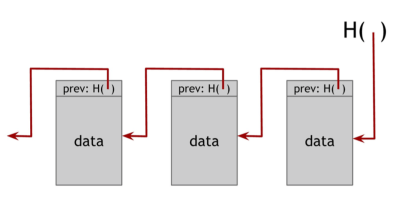
\includegraphics[width=0.8\textwidth]{cadena_de_bloques.png}
     \caption{\textit{Blockchain}: lista enlazada de bloques construida con apuntadores hash. Fuente: \textit{Bitcoin and Cryptocurrency Technologies Book. Princeton University}.\cite{narayanan2016bitcoin}}
    \label{blockchain_linkedlist}
\end{figure}


Desde el punto de vista de negocios, el \textit{blockchain} se  define como una plataforma de tipo \textit{P2P} (por sus siglas en inglés Peer-to-Peer),  mediante la cual los pares pueden intercambiar valores usando transacciones sin la necesidad de un árbitro central de confianza. Esto permite que \textit{blockchain} sea un mecanismo de consenso descentralizado donde ninguna autoridad única está a cargo de la base de datos~\cite{bashir2017mastering}.

Dadas las características y propiedades antes expuestas, la tecnología \textit{blockchain}  se adapta especialmente a escenarios en los que se requiera almacenamiento cronológico de datos, inmutables y cuya confianza no prevalezca en un ente central de control, sino en los participantes involucrados~\cite{wiki:CadenaBloques}.

Dentro de los elementos generales que debería contener cualquier plataforma \textit{blockchain} se encuentran:
\begin{itemize}
    \item Direcciones: las direcciones son identificadores únicos que se utilizan en una transacción dentro del \textit{blockchain} para designar remitentes y destinatarios. Una dirección generalmente es una clave pública. Si bien las direcciones pueden ser reutilizadas por el mismo usuario, las direcciones son únicas. En la práctica, sin embargo, un solo usuario no puede usar la misma dirección nuevamente y generar una nueva para cada transacción. 
    \item Transacción: Una transacción es la unidad fundamental del \textit{blockchain}. Una transacción representa una transferencia de valor de una dirección a otra.
    \item Bloque: Un bloque se compone de varias transacciones y otros elementos como el {\it hash} del bloque anterior ({\it hash pointer}), {\it marca de tiempo} y {\it banderas(bits predefinidos que contienen valores binarios)}.
    \item Red punto-a-punto (P2P): ésta es una topología de red mediante la cual todos los compañeros (nodos de la red) se pueden comunicar entre sí y enviar y recibir mensajes.
    \item {\it Scripting} o lenguaje de programación: los {\it scripts} de transacción son conjuntos de comandos predefinidos para que los nodos transfieran tokens de una dirección a otra y realicen otras funciones. Una característica deseable de los lenguajes utilizados dentro del \textit{blockchain} es que sean “Turing completos”.
    \item Contratos Inteligentes: programas que se ejecutan sobre el \textit{blockchain} y encapsulan la lógica de negocios que se ejecutará cuando se cumplan ciertas condiciones. La función de contrato inteligente no está disponible en todas las cadenas de bloques, pero ahora se está convirtiendo en una característica muy deseable debido a la flexibilidad y la potencia que proporciona a las aplicaciones \textit{blockchain}.
    \item Máquina Virtual: Una máquina virtual permite que el código Turing completo se ejecute en el \textit{blockchain} (como contratos inteligentes), a diferencia  de un {\it script} de transacción que puede estar limitado en su funcionamiento. Las máquinas virtuales no están disponibles en todas las plataformas  \textit{blockchains}; sin embargo, varios plataformas actuales usan máquinas virtuales para ejecutar programas, por ejemplo, Ethereum Virtual Machine (EVM) y Chain Virtual Machine (CVM).
    \item Nodos: Un nodo en una red \textit{blockchain} realiza varias funciones dependiendo del rol que desempeña. Un nodo puede proponer y validar transacciones y realizar operaciones de minería para facilitar el consenso y asegurar la plataforma \textit{blockchain}. Esto se hace siguiendo un protocolo o algoritmos de consenso explicados a continuación. Los nodos también pueden realizar otras funciones, como la verificación simple de pagos (nodos livianos), validadores y muchas otras funciones según el tipo de \textit{blockchain} utilizada y el rol asignado al nodo.
\end{itemize}

\textbf{Características principales}
\begin{itemize}
    \item Consenso Distribuido: El consenso distribuido es el principal soporte de una plataforma \textit{blockchain}. Esto permite que el \textit{blockchain} presente una única versión de la verdad acordada por todas las partes sin el requisito de una autoridad central.
    \item Verificación de transacciones: Todas las transacciones publicadas por los  nodos en el \textit{blockchain} se verifican en base a un conjunto predeterminado de reglas y sólo se seleccionan las transacciones válidas para su inclusión en un bloque.
    \item Transferencia de valores entre pares: El \textit{blockchain} permite la transferencia de valor entre sus usuarios a través de tokens(unidad de valor que una organización crea para gobernar su modelo de negocio). Se puede pensar que los tokens son portadores de valor.
    \item Generación de criptomonedas: En un \textit{blockchain} se  puede generar criptomonedas como un incentivo para sus mineros que validan las transacciones y gastan recursos para asegurar la plataforma. Esta es una función opcional según el tipo de \textit{blockchain} utilizado.
    \item Propiedad intelectual: Es posible vincular un elemento digital o físico al \textit{blockchain} de una manera irrevocable, de modo que no pueda ser reclamado por nadie más; el propietario tiene el control total de su activo y no puede ser gastado doblemente o tener doble propiedad. Esta característica tiene implicaciones de gran alcance, especialmente en la gestión de derechos digitales y en los sistemas electrónicos de efectivo, donde la detección de doble gasto es un requisito clave
    \item Proveedor de seguridad: El \textit{blockchain} se basa en una tecnología criptográfica comprobada que garantiza la integridad y la disponibilidad de los datos. Generalmente, la confidencialidad no se proporciona en primera instancia debido a los requisitos de transparencia(transacciones publicas y visibles para cualquier usuario asociado o no la red blockchain), sin embargo la investigación en esta área ha  madurado y se ha avanzado mucho para obtener confidencialidad y privacidad en las plataformas \textit{blockchain} que necesiten de estas características.
    \item Inmutabilidad: Otra característica clave de \textit{blockchain} es el hecho que los registros que se agregan una vez a la plataforma son inmutables. Aunque teóricamente existe la posibilidad de revertir los cambios, en la práctica se considera casi imposible de lograr, ya que se requiere de una cantidad inaccesible de recursos informáticos, ya que se tendría que accesar a cada uno de los nodos que comparten el registro, alterar cada una de sus decisiones y todo esto en simultaneo, necesitando gran poder de computo para cumplir dicho objetivo.
    \item Unicidad: Esta característica del \textit{blockchain} garantiza que cada transacción sea única y no se haya consumido anteriormente. Esto es especialmente relevante en las plataformas \textit{blockchain} de criptomonedas donde la detección y  evasión  del “doble gasto” son un requisito clave.
\end{itemize}

La Figura~\ref{blockchain_properties} muestra las características de la tecnología \textit{blockchain}.

\begin{figure}[h]
    \centering
    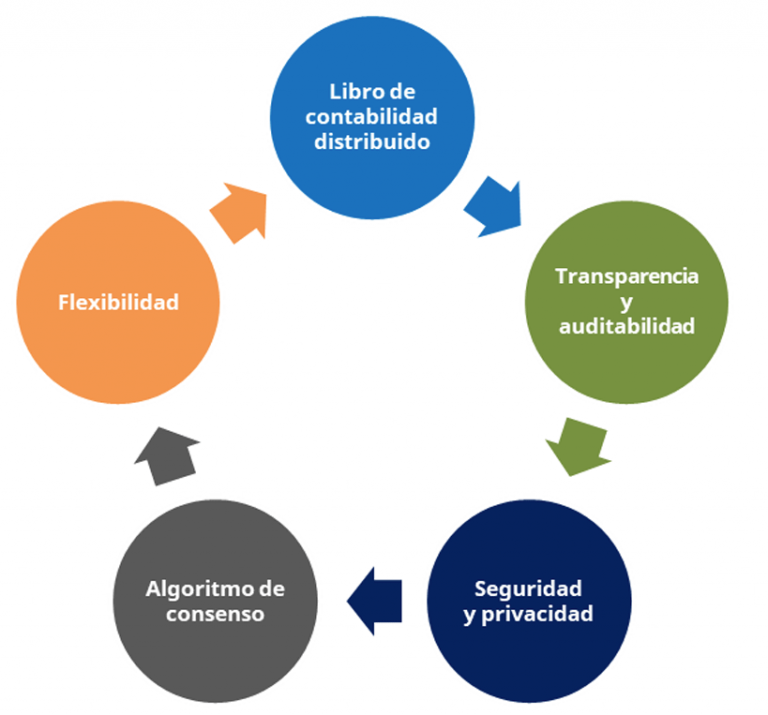
\includegraphics[width=0.5\textwidth]{caracteristicas_blockchain.png}
     \caption{Caracertisticas principales de la tecnologia \textit{blockchain} }
    \label{blockchain_properties}
\end{figure}



\textbf{Tipos de plataformas \textit{blockchain}}:  Basado en la evolución del \textit{blockchain} en los últimos años, esta tecnología se puede dividir en varios tipos con atributos distintos que en muchos casos suelen solaparse:

\begin{itemize}
    \item Públicos:  Estos  tipos de \textit{blockchain}s están abiertos al público y cualquiera puede participar como un nodo en el proceso de toma de decisiones y éstos  pueden o no ser recompensados por su participación. Los registros son propiedad de nadie y están públicamente abiertos para que cualquier persona participe y consulte. Todos los usuarios  mantienen una copia del \textit{blockchain} en sus nodos locales y utilizan un mecanismo de consenso distribuido para tomar una decisión sobre el eventual estado del mismo. Este tipo  también se conocen como libros no permisados.
    \item Privadas: Como su nombre lo indica son privadas y están abiertas sólo a un consorcio o grupo de individuos u organizaciones que han decidido compartir el libro de contabilidad entre ellos.
    \item Semi-privadas: En este tipo de plataformas \textit{blockchain}, una parte del mismo es privada y la otra es pública. La parte privada está controlada por un grupo de individuos, mientras que la parte pública está abierta para la participación de cualquier persona.
    \item Libros contable autorizado: Un libro de contabilidad autorizado es un \textit{blockchain} por el cual los participantes de la red son conocidos y de confianza. Los libros mayores autorizados no necesitan usar un mecanismo de consenso distribuido, en su lugar se puede usar un protocolo de acuerdo para mantener una versión compartida de la verdad sobre el estado de los registros en el \textit{blockchain}. Tampoco es obligatorio que una plataforma \textit{blockchain} autorizada sea privada, ya que puede ser un \textit{blockchain} público, pero con control de acceso regulado.
    \item Libros contable distribuido: Este libro se distribuye entre sus participantes y se extiende a través de múltiples sitios u organizaciones. Este tipo puede ser privado o público. La idea clave es que, a diferencia de muchas otras plataformas \textit{blockchain}, los registros se almacenan de forma contigua en lugar de ordenarse en bloques.
    \item Tokenisadas: Son \textit{blockchain}s estándar que generan criptomonedas como resultado de un proceso de consenso a través de la minería o mediante la distribución inicial. Aquí entra cualquier plataforma relacionada a criptomonedas.
\end{itemize}

\subsection {Sistemas distribuidos}

Primeramente es necesaria la  comprensión de los sistemas distribuidos porque  la tecnología de \textit{blockchain} en su núcleo es un sistema distribuido, específicamente, un sistema distribuido descentralizado.

Los sistemas distribuidos son un paradigma informático mediante el cual dos o más nodos trabajan entre sí en una manera coordinada para lograr un resultado común y está modelada de tal manera que los usuarios finales lo ven como una única plataforma lógica~\cite{bashir2017mastering}.

Se define un nodo como un jugador individual en un sistema distribuido. Todos los nodos son capaces de enviar y recibir mensajes hacia y desde un nodo a otro. Cada nodo posee memoria y procesador propios y se clasifican en tres tipos:  honestos, defectuosos y maliciosos.
%, poseen  memoria y procesador propios. 
Un nodo que puede mostrar un comportamiento arbitrario también se conoce como nodo bizantino. Este comportamiento arbitrario puede ser intencionalmente malicioso, lo cual es perjudicial para el funcionamiento de la red. En general, cualquier comportamiento inesperado de un nodo en la red se puede categorizar como nodo bizantino.

El principal desafío que se presenta en los sistemas distribuidos es la coordinación entre nodos y tolerancia a fallas. Si algunos de los nodos se vuelven defectuosos o se rompen enlaces de red, el sistema distribuido debería ser capaz de  tolerar este tipo de situación y mantener su funcionamiento sin problemas para lograr el resultado deseado.


\subsection{Consenso}
El consenso es un proceso de acuerdo entre nodos desconfiados sobre un estado final de datos. Para lograr el consenso, se pueden usar diferentes algoritmos. En general es fácil llegar a un acuerdo entre dos nodos (por ejemplo en esquemas cliente-servidor) pero cuando múltiples nodos participan en un sistema distribuido y necesitan ponerse de acuerdo en un solo valor, se vuelve complejo lograr dicho consenso. El concepto que define la obtención de consenso entre nodos múltiples se conoce como consenso distribuido (ver Figura~\ref{blockchain_consensus})~\cite{bashir2017mastering}. 

\begin{figure}[h]
    \centering
    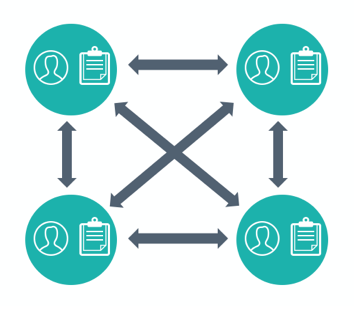
\includegraphics[width=0.4\textwidth]{consenso-nodos.png}
     \caption{Ejemplo de nodos efectuando consenso}
    \label{blockchain_consensus}
\end{figure}

\textbf{Mecanismos de consenso:}  Un mecanismo de consenso es un conjunto de pasos que toman todos, o la mayoría de los nodos, para acordar un estado o valor propuesto~\cite{swanson2015consensus}. Los mecanismos de consenso han pasado recientemente a ser el centro de atención y ganó mucha popularidad con el advenimiento de la primera implementación pública de \textit{blockchain}, la famosa plataforma Bitcoin \cite{nakamoto2008bitcoin}.

Existen cinco requisitos que deben cumplirse para proporcionar los resultados deseados en un mecanismo de consenso:

\begin{itemize}
\item Acuerdo: todos los nodos confiables deciden sobre el mismo valor.
\item Terminación: todos los nodos confiables terminan la ejecución del proceso de consenso y eventualmente llegan a una decisión.
\item Validez: el valor acordado por todos los nodos honestos debe ser el mismo que el valor inicial propuesto por al menos un nodo confiable.
\item Tolerante a fallas: el algoritmo de consenso debería poder ejecutarse en presencia de fallas o nodos maliciosos (nodos bizantinos).
\item Integridad: este es un requisito donde ningún nodo toma la decisión más de una vez. Los nodos toman decisiones solo una vez en un solo ciclo de consenso.
\end{itemize}

Existen varios tipos de mecanismo de consenso, dentro de los dos mas comunes encontramos:
%, dentro de los 2 mas comunes encontramos:
\begin{itemize}
\item Basados en la tolerancia a fallas bizantinas: sin operaciones de cálculo intensivo, como la inversión de hash parcial, este método se basa en un esquema simple de nodos que publican mensajes firmados. Eventualmente, cuando se recibe una cierta cantidad de mensajes, se llega a un acuerdo. Una de las implementaciones más famosas de este tipo, es  el  algoritmo Paxos publicado por Leslie Lamport~\cite{lamport2001paxos}.

\item Basados en líderes: este tipo de mecanismo requiere que los nodos compitan por la lotería de elección de líderes y el nodo que los gana proponga un valor final. Dentro de las implementaciones conocidas de este tipo, destaca el protocolo RAFT publicado por Diego Ongaro y John Ousterhout~\cite{ongaro2015raft}.
\end{itemize}

El concepto de consenso de sistemas distribuidos ha sido incorporado  en la tecnología \textit{blockchain} para proporcionar un medio de aceptación y validación única de la verdad por parte de todos los pares en la red \textit{blockchain}. Dentro de los \textbf{algoritmos de consenso} más importantes que están disponibles hoy o están siendo investigados en el contexto de \textit{blockchain} sobresalen:

\begin{itemize}
\item Prueba de trabajo: este tipo de mecanismo de consenso se basa en la prueba del consumo de recursos computacionales suficientes  antes de proponer un valor para su aceptación por parte de la red. Este mecanismo es utilizado en la plataforma Bitcoin  y otras plataformas \textit{blockchain} asociadas a criptomonedas.
\item Prueba de apuesta: este algoritmo funciona con la idea de que un nodo o usuario tiene una apuesta suficiente en el sistema; por ejemplo, el nodo ha invertido los recursos suficientes  para que cualquier intento de  perjudicar o comprometer a la red concluiria en una perdida de sus propios recursos invertidos. Esta idea fue presentada por el proyecto de Peercoin y se encuentra en etapa de prueba  en el \textit{blockchain} de Ethereum. Otro concepto importante en este tipo de algoritmo es la “edad de la moneda”, que es un derivado desde la cantidad de tiempo y la cantidad de monedas que no se han gastado. En este modelo, las posibilidades de proponer y firmar el siguiente bloque aumentan con la edad de la moneda.
\item Prueba de importancia: esta prueba comparte similitud con la “Prueba de Apuesta” sin embargo este mecanismo no solo se basa en la cantidad de  apuesta que tiene un usuario en el sistema, sino que adicionalmente monitorea el uso y movimiento de los tokens por parte del usuario para establecer un nivel de confianza e importancia. Este mecanismo es utilizado en el proyecto Nemcoin.
\item Prueba de tiempo transcurrido: introducido por Intel, usa un Entorno Confiable de Ejecución (TEE por sus siglas en inglés) para proporcionar aleatoriedad y seguridad en el proceso de elección del líder a través de un tiempo de espera garantizado. Requiere el Intel SGX (Software Guard Extension) procesador para proporcionar la garantía de seguridad\cite{costan2016intel}.
\item Consenso federado o consenso bizantino federado: los nodos en este protocolo mantienen un grupo de pares y compañeros de confianza pública y propaga sólo aquellas transacciones que han sido validadas por la mayoría de los nodos de confianza. Usados en el protocolo de consenso del proyecto Stellar\cite{stellarProject:stellarBasics}
\item Mecanismos basados  en reputación: mecanismo donde un líder es elegido sobre la base de la reputación que ha construido con el tiempo en la red. Esto puede basarse en la votación de otros miembros.
\end{itemize}


%!TEX root = ../thesis.tex

\section{Descentralizacion}  %Title of the First Chapter

La descentralización se ha utilizado en  estrategia, gestión y gobierno durante mucho tiempo. La idea básica consiste en distribuir el control y la autoridad a las periferias en lugar de que una autoridad central tenga el control total de la organización. Esto resulta en varios beneficios para las organizaciones, como una mayor eficiencia, una toma de decisiones más rápida, y una menor carga para la gerencia de bajo y alto nivel~\cite{bashir2017mastering}.

A pesar de no ser un concepto nuevo, la descentralización empieza a tomar gran importancia en el mundo tecnológico, al ser el servicio principal y central brindado por plataformas \textit{blockchain}. Si bien los sistemas descentralizados  y distribuidos tienen mucho en común su principal diferencia radica en que, en los sistemas distribuidos todavía existe una autoridad central que gobierna todo el sistema, mientras que en un sistema descentralizado, no existe tal autoridad. Se podría decir que el \textit{blockchain} es la manera perfecta de proveer una  plataforma que no necesite ningún intermediario o entidad de control, y puede funcionar mediante la interacción de varios participantes o nodos, los cuales definen o validan el estado actual del sistema mediante mecanismos de consenso, específicamente mecanismos de consenso descentralizados que son una verdadera innovación en el paradigma descentralizado. La Figura~\ref{blockchain_descentralziation} compara los tres tipos de redes.

\begin{figure}[h]
    \centering
    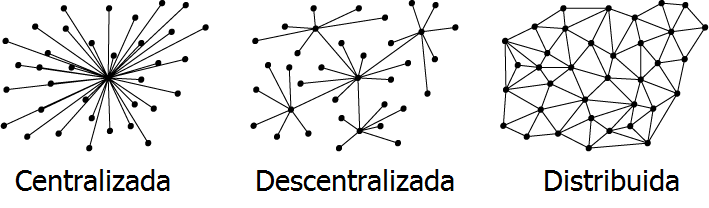
\includegraphics[width=0.8\textwidth]{descentralizacion.png}
     \caption{Diferencia entre redes centralizadas, descentralizadas y distribuidas}
    \label{blockchain_descentralziation}
\end{figure}

Existen dos métodos de descentralización conocidos que pueden ser utilizados:
\begin{itemize}
    \item Desintermediación: El término es bastante común y de uso frecuente en economía e implica la eliminación de intermediarios en una cadena de suministro, o la eliminación de los intermediarios en relación con una transacción o una serie de transacciones~\cite{lin2015infinite}. Un ejemplo de este término aplicado al \textit{blockchain} es la famosa plataforma Bitcoin, en donde se puede  enviar dinero (token) a un conocido, amigo o familiar con solo saber su dirección, eliminando la  necesidad de que una o varias entidades bancarias validen y realicen la transferencia hasta la cuenta destino.
    \item Por competencia:  En este método, un grupo de proveedores de servicios compiten entre sí para ser seleccionados por el sistema para la prestación de servicios. Este paradigma no logra la descentralización completa, pero en cierta medida asegura que un intermediario o proveedor de servicios no esté monopolizando el mismo. En el contexto de tecnología \textit{blockchain}, se puede prever un sistema en el cual los contratos inteligentes pueden elegir un proveedor de datos o nodo candidato externo de una gran lista de proveedores en función de su reputación, puntaje previo, revisiones y calidad del servicio. Esto no dará lugar a una descentralización completa, pero permite que los contratos inteligentes hagan una elección libre en base a los criterios mencionados anteriormente. De esta forma, se crea un entorno de competencia entre los proveedores de servicios, en el que compiten entre sí para convertirse en el proveedor de datos de elección~\cite{bashir2017mastering}.
\end{itemize}

Existe un marco de trabajo que se puede  utilizar para evaluar los requisitos de descentralización de una variedad de elementos en el contexto de la tecnología \textit{blockchain} y que fue propuesto por Arvind Narayanan entre otros~\cite{narayanan2012critical}. El marco básicamente propone cuatro preguntas que se deben responder para generar una idea clara de cómo se puede descentralizar un sistema:
\begin{enumerate}
    \item ¿Qué está siendo descentralizado?
Hace referencia al sistema que se está descentralizando o se quiere descentralizar.
    \item ¿Qué nivel de descentralización se requiere?
Se responde especificando el nivel de descentralización requerido, el cual puede ser aplicando a alguno de los dos métodos discutidos anteriormente: Desintermediacion (descentralizacion total) o Por Competencia (descentralización parcial).
    \item ¿Qué \textit{blockchain} se usa?
Selección de plataforma \textit{blockchain}  adecuada para una aplicación en particular.
    \item ¿Qué mecanismo de seguridad se usa?
Finalmente, es necesario responder a una pregunta clave sobre el mecanismo de seguridad,  en otras palabras cómo se puede garantizar la seguridad de un sistema descentralizado. Un buen ejemplo de esto puede ser la Atomicidad, por el cual la transacción se ejecuta por completo o no se ejecuta en absoluto. El objetivo es asegurar la integridad del sistema.
\end{enumerate}

\subsection{Tipos de organismos descentralizados}
\begin{itemize}
    \item Las organizaciones descentralizadas (DOs, por sus siglas en inglés de {\it Descentralized Organizations})  son programas de software que se ejecutan en una \textit{blockchain} y requiere la interacción constante entre personas o integrantes de la organización para efectuar funciones y operaciones relacionadas a la lógica de negocios. Una vez que una DO, en la forma de un contrato inteligente o un conjunto de contratos inteligentes, se agrega al \textit{blockchain}, el mismo se descentraliza y las partes interactúan entre sí en función del código definido en el software de DO.
    \item Las organización autónoma descentralizada (DAO, por sus siglas en inglés {\it Decentralized Autonomous Organizations})  es básicamente lo mismo que una DO con la diferencia principal que las DAO son autónomos, lo que significa que son completamente automáticos y contienen una lógica artificialmente inteligente, mientras que los DO carecen de esta característica y dependen de los datos humanos para ejecutar la lógica comercial.
    \item Las corporaciones autónomas descentralizadas (DAC, por sus siglas en inglés {\it Decentralized Autonomous	Corporations}) son un concepto similar, pero se consideran un subconjunto de las  DAO. Las definiciones de DAC y DAO se pueden superponer en varios escenarios, sin embargo usualmente difieren en  que los DAO en general se consideran sin fines de lucro, mientras que los DAC pueden ganar dinero a través de acciones ofrecidas a los participantes y mediante el pago de dividendos. Estas corporaciones pueden ejecutar un negocio automáticamente sin intervención humana en función de la lógica programada dentro de ellos.
    \item Las sociedades autónomas descentralizadas (DAS, por sus siglas en inglés {\it Decentralized Autonomous	Societies}) son un concepto mediante el cual sociedades enteras pueden funcionar en un \textit{blockchain} con la ayuda de múltiples contratos inteligentes complejos y una combinación de DAO y aplicaciones descentralizadas (DAPP, por sus siglas en inglés {\it Decentralized	Application}) que funcionan de forma autónoma. Este modelo no significa un enfoque fuera de la ley, ni se basa en una ideología totalmente libertaria; en cambio, muchos servicios que ofrece un gobierno se pueden entregar a través del \textit{blockchain}, como sistemas de tarjetas de identidad del gobierno, emisión de pasaportes y registros de escrituras, matrimonios y nacimientos.
    \item Las aplicaciones descentralizadas (DAPP) son programas de software que pueden ejecutarse en su propia \textit{blockchain}, utilizar otra \textit{blockchain}  o utilizar sólo protocolos de una solución de \textit{blockchain} existente. Todas los DAO, DAC y DO son básicamente aplicaciones descentralizadas que se ejecutan en la parte superior de un \textit{blockchain} en una red punto a punto. Este es el último avance en tecnología con respecto a la descentralización.

\end{itemize}
%!TEX root = ../thesis.tex

\section {Criptografia en Blockchain}  %Title of the First Chapter

%\textcolor{red}{Me parece que el término correcto es crifra, en lugar de encriptar. Verificar.}
%\textcolor{blue} {encriptar cambiado por cifrar en varias partes del parrafo, verificar si es la correcion sugerida. Link de referencia: http://red.computerworld.es/actualidad/cuando-alguien-dice-encriptar-y-quiere-decir-cifrar}

La criptografía es la ciencia encargada del estudio de los algoritmos, protocolos y sistemas que se utilizan para dotar de seguridad a las comunicaciones, a la información y a las entidades que se comunican~\cite{pastor1998criptografia}.

El método en general implica tomar datos sin cifrar, como una pieza de texto, y cifrarlos usando un algoritmo matemático. Esto produce un texto cifrado, una información que es completamente inútil y sin sentido, hasta que se descifra con la ayuda de una clave preestablecida y conocida solamente por el emisor y receptor. Este método  criptográfico se conoce como criptografía de llave simétrica (ver Figura~\ref{blockcain_llavesimetrica}).

\begin{figure}[h]
    \centering
    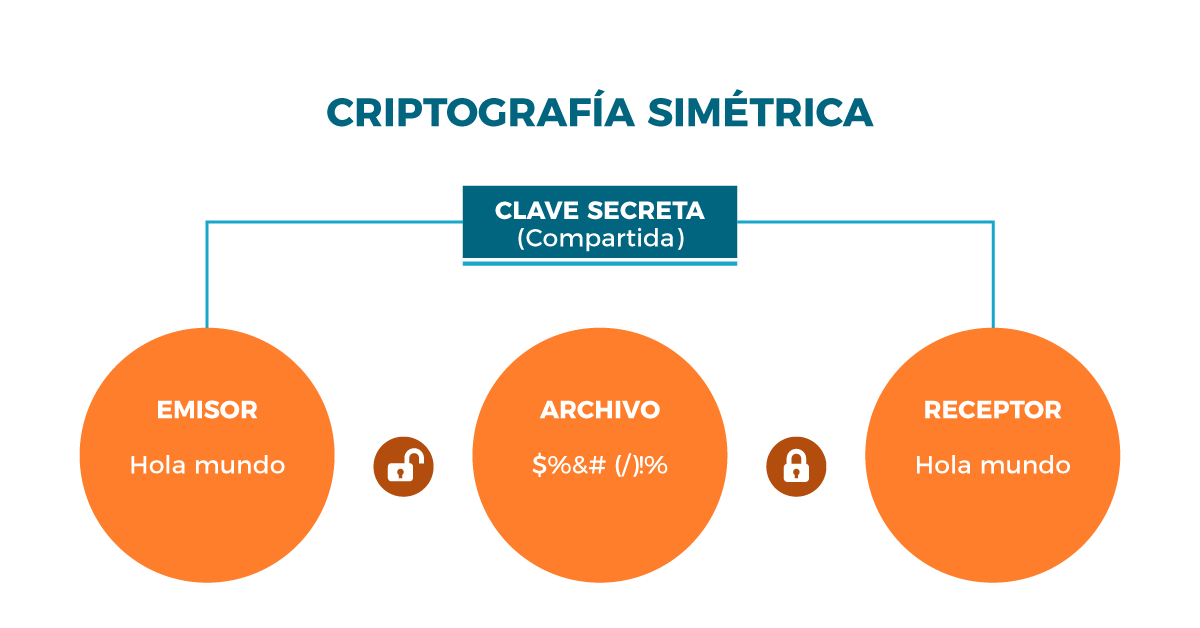
\includegraphics[width=0.7\textwidth]{cripto_simetrica.png}
     \caption{Método criptografico de llave simétrica} 
    \label{blockcain_llavesimetrica}
\end{figure}

La criptografía proporciona varios servicios de seguridad, los cuales son vitales y necesarios en tecnología \textit{blockchain} o cualquier plataforma que haga uso de la misma~\cite{bashir2017mastering}:

\begin{itemize}
    \item \textbf{Confidencialidad} es la garantía de que la información solo está disponible para las entidades autorizadas.
    \item \textbf{Integridad} es la garantía de que la información es modificable sólo por entidades autorizadas.
    \item \textbf{Autenticación} proporciona seguridad sobre la identidad de una entidad o la validez de un mensaje. Hay dos tipos de autenticación:
    La \textbf{autenticación de la entidad} es la garantía de que una entidad está actualmente involucrada y activa en una sesion de comunicacion.
    La \textbf{autenticación de origen de datos}  es la garantía de verificación sobre la fuente de información, esta  implica la integridad de los datos ya que si  una fuente ha sido corroborada, se asegura que los datos no han sido alterados. Diversos métodos, como los códigos de autenticación de mensajes (MAC, por sus siglas en ingles  Message Authentication Code) y las firmas digitales son los más comúnmente utilizados.
    \item \textbf{No repudio}  es la  garantía de que una entidad no puede negar un compromiso o acción previa proporcionando evidencia. El uso de criptografía garantiza que este servicio produce evidencias infalibles e irrefutables  en transacciones electrónicas para que, en caso de disputas, se pueda utilizar como confirmación de una acción.
    \item \textbf{Rendición de Cuentas} es la garantía de que las acciones que afectan la seguridad de la plataforma se pueden rastrear hasta la fuente responsable. Esto generalmente es proporcionado por los mecanismos de registro y auditoría en los sistemas donde se requiere una auditoría detallada debido a la naturaleza del negocio.
\end{itemize}
 
\subsection {Criptografía de llave pública}

A pesar de estar basado en un marco similar, el tipo de criptografía utilizado en \textit{blockchain} es conocida como \textbf{criptografía de llave pública} o \textbf{criptografía asimétrica}, este tipo representa una mejora en la criptografía de llave simétrica estándar, ya que permite que la información se transfiera a través de una llave pública que se puede compartir con cualquier persona~\cite{liskacademy:blockchainCryptographyExplained}.

En la práctica el remitente cifra los datos usando la llave pública del destinatario y luego los transmite a través de la red al receptor. Una vez que llega al receptor, se puede descifrar usando la llave privada del receptor. De esta manera, la llave privada permanece en el lado del receptor y no hay necesidad de compartir llaves para realizar el cifrado y descifrado, que es lo que ocurre en el cifrado simétrico. La Figura~\ref{blockcain_llaveasimetrica} muestra gráficamente este proceso.

Adicionalmente, a través de la criptografía de llave pública se produce una firma digital que garantiza la integridad de los datos que se muestran. Esto se hace combinando la llave privada de un usuario con los datos que desean firmar, a través de un algoritmo matemático.

\begin{figure}[h]
    \centering
    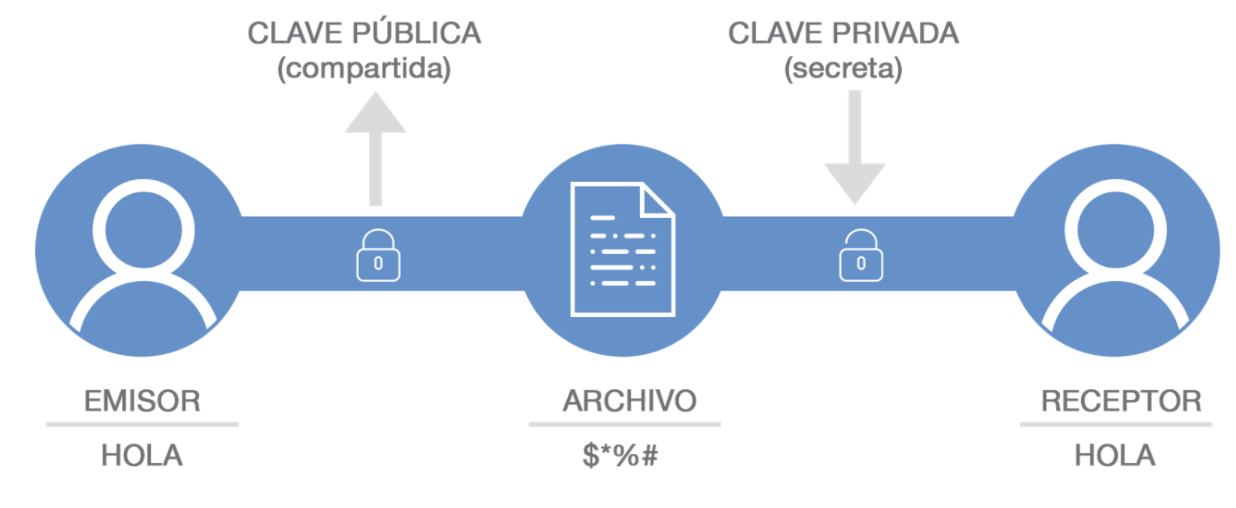
\includegraphics[width=0.7\textwidth]{cripto_asimetrica.png}
     \caption{Método criptográfico de llave asimétrica} 
    \label{blockcain_llaveasimetrica}
\end{figure}

\subsection{Firmas digitales}

Las firmas digitales proporcionan un medio para asociar un mensaje con una entidad desde la cual se originó . Las firmas digitales se usan para proporcionar integridad, autenticación de origen de datos y no repudio.

Dentro de las firmas digitales encontramos 3 propiedades importantes a resaltar, la autenticidad, imposibilidad de force y la no reutilización. Autenticidad significa que las firmas digitales son verificables por una parte receptora. La  imposibilidad de force garantiza que solo el remitente del mensaje pueda usar la funcionalidad de firma con la llave privada y finalmente la no reutilización significa que la firma digital no se puede separar de un mensaje para ser utilizado en otro distinto.

Las firmas digitales son creadas a partir de tres algoritmos cuya finalidad radica en 
hacer absolutamente imposible calcular la llave privada en función de la clave pública o de los datos cifrados y garantizar la autenticidad de una firma basada en el mensaje y la llave privada, verificada a través de la clave pública. A continuación  se describen brevemente los algoritmos:
\begin{itemize}
    \item Un algoritmo de generación de claves, que proporciona una llave privada y pública.
    \item Un algoritmo de firma que combina datos y llave privada para hacer una firma.
    \item Un algoritmo que verifica las firmas y determina si el mensaje es auténtico o no en función del mensaje, la clave pública y la firma.
\end{itemize}

\subsection{Hashing}

Hashing es el proceso de tomar una entrada de cualquier longitud y convertirla en una salida criptográfica fija a través de un algoritmo matemático (Bitcoin usa SHA-256, por ejemplo). Los ejemplos de tales entradas pueden incluir desde un pequeño fragmento de información, como un mensaje hasta un gran caché de información variable, como un bloque de transacciones~\cite{liskacademy:blockchainCryptographyExplained}. La Figura~\ref{blockcain_hashing} ilustra el mecanismo de hashing.

\begin{figure}[h]
    \centering
    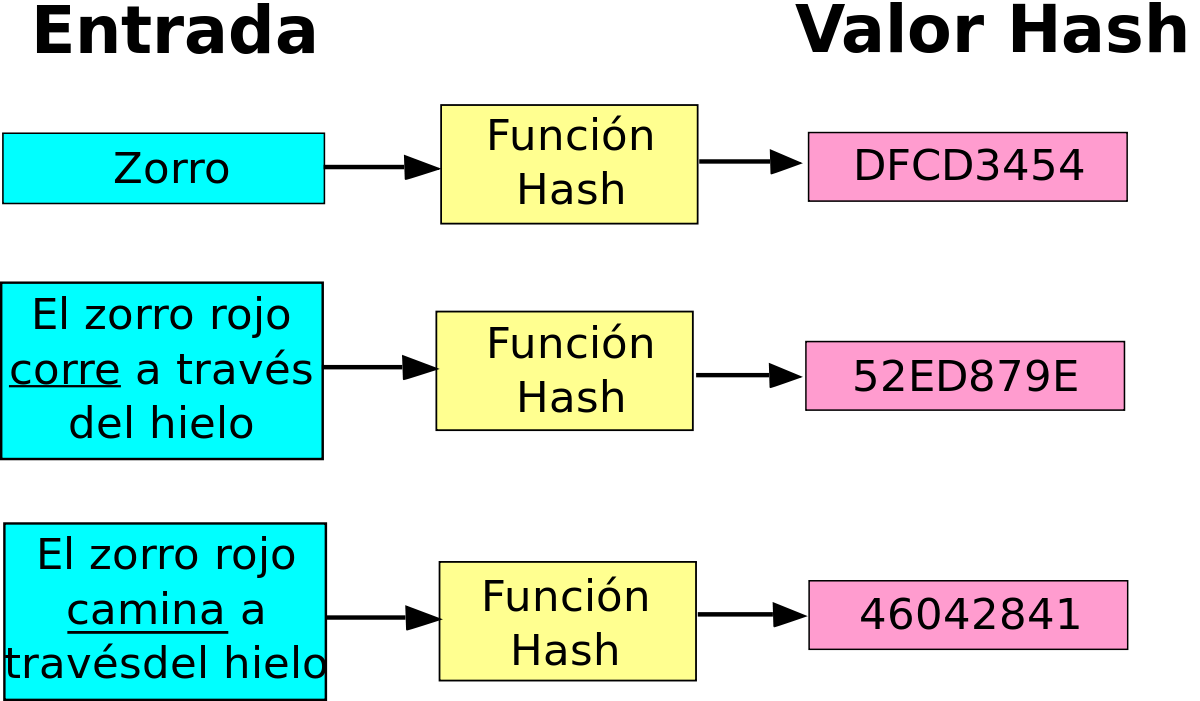
\includegraphics[width=0.6\textwidth]{hashing.png}
     \caption{Ilustración de mecanismo hashing} 
    \label{blockcain_hashing}
\end{figure}

El hashing aumenta drásticamente la seguridad de los datos ya que cualquiera que intente descifrar los datos mirando  el código  hash no podrá calcular la longitud de la información cifrada en función del hash mencionado. Una función de hash criptográfica debe tener varias cualidades cruciales para ser considerada útil:
\begin{itemize}
    \item Imposible producir el mismo valor hash para diferentes entradas.
    \item El mismo mensaje siempre producirá el mismo valor hash.
    \item Rápido en  la  generacion de un hash para cualquier mensaje dado.
    \item Imposible determinar la entrada en función del valor hash.
    \item Incluso el más mínimo cambio a una entrada altera por completo el hash.
\end{itemize}

En \textit{blockchain}, los hashes se usan para representar el estado actual del mundo, o para ser más precisos, el estado del \textit{blockchain}. La entrada representa todo lo que ha sucedido en el \textit{blockchain}, es decir, cada transacción realizada hasta ese punto combinada con los nuevos datos que se agregan.

Como se mencionó, el más mínimo cambio en cualquier parte de la entrada da como resultado un gran cambio en la salida; en esto radica la seguridad irrefutable de la tecnología \textit{blockchain}. Cambiar cualquier registro que haya sucedido previamente en un \textit{blockchain} cambiaría todos los hashes, haciéndolos falsos y obsoletos. Esto se vuelve imposible cuando se toma en cuenta la naturaleza transparente de \textit{blockchain}, ya que estos cambios deberían realizarse a plena vista de toda la red y en todos los nodos que la conforman.

El primer bloque de una cadena de bloques, conocido como bloque de génesis, contiene sus transacciones que, cuando se combinan y validan, producen un hash único. Este hash y todas las transacciones nuevas que se están procesando se usan luego como entrada para crear un nuevo hash que se usa en el siguiente bloque de la cadena. Esto significa que cada bloque se vincula a su bloque anterior a través de su hash, formando una cadena de regreso al bloque de génesis, de ahí el nombre \textit{blockchain}. De esta forma, las transacciones se pueden agregar de forma segura siempre que los nodos de la red estén en consenso sobre cuál debería ser el hash.



\section {Plataformas Blockchain}

En la actualidad, existe una amplia gama de proyectos de código abierto disponibles para la creación de aplicaciones utilizando la tecnología \textit{blockchain}. Aunque la mayor parte de éstos se encuentran relacionados a proyectos de criptomonedas, cada vez más empresas y organizaciones estudian su aplicación en escenarios distintos al del ''dinero digital'', con la finalidad de obtener beneficios (estudiados en secciones anteriores) como por ejemplo, soluciones en cadena de suministros, gestión de propiedad intelectual, administración de procesos de negocio, control de acceso e incluso plataformas de votaciones.

En esta sección se exponen dos de las plataformas más populares y estables en cuanto a documentación, trayectoria, comunidad y soporte se refiere: Ethereum e IBM Hyperledger Fabric. Ambas ofrecen un marco de trabajo (framework) ideal para el desarrollo de aplicaciones basadas en \textit{blockchaion} o DLT (por sus siglas en inglés {\it Distributed Ledger Tecnology}). Asimismo, se presenta una descripción de cada una de las tecnologías y finalmente se definen y comparan sus principales características. 


\subsection{Ethereum}
Ethreum es una red de \textit{blockchain} \textbf{pública} que posee además una criptomoneda denominada \textit{Ether}; también puede ser definida como una plataforma de código abierto que permite a los desarrolladores construir e implementar aplicaciones descentralizadas. Ethereum fue propuesto por Vitalik Buterin a finales de 2013~\cite{wood2014ethereum}, sin embargo fue lanzado oficialmente en julio de 2015. Ha ganado popularidad como plataforma de elección para muchas aplicaciones (DAPP's), así como para la creación y lanzamiento de ICO's (por sus siglas en inglés {\it Initial Coin Offering}). 

Ethereum, cuenta también con la posibilidad de creación de contratos inteligentes que definen reglas y sanciones en torno a un acuerdo, haciendo cumplir obligaciones establecidas en el mismo. En Ethereum, dichos contratos se tratan como {\it scripts} autónomos o aplicaciones descentralizadas (DAPP's) que poseen un estado que se almacena en el \textit{blockchain} para su posterior ejecución. Para su desarrollo, es posible elegir entre varios lenguajes, siendo Solidity el más recomendado. El mecanismo de consenso de Ethereum está basado en la  ''prueba de trabajo'', sin embargo, está previsto cambiarlo por la ''prueba de apuesta'', cual se encuentra en fase de prueba.

Finalmente, Ethereum utiliza una máquina virtual (EVM, por sus siglas en inglés {\it Ethereum Virtual Machine}), es decir, una computadora global distribuida donde se ejecutan todos los contratos inteligentes. Las operaciones efectuadas dentro del EVM, son ejecutadas simultáneamente por cada nodo de la red; por esta razón existe un mecanismo para limitar los recursos utilizados en cada contrato, conocido como \textit{gas}. Cada una las operaciones realizadas tiene un costo medido en gas, y cada unidad de gas consumida por una transacción debe ser pagada en \textit{Ether}.

\subsection{Hyperledger Fabric} 
Hyperledger Fabric es un proyecto avalado e impulsado por \textit{The Linux Foundation} y es mantenido actualmente por IBM~\cite{androulaki2018hyperledger}. Consiste en una infraestructura \textit{blockchain} autorizada de código abierto que proporciona una arquitectura modular y a su vez cuenta con una distinción de roles entre nodos, la cual permite la  ejecución de contratos inteligentes y servicios configurables de consenso y membresía. 

Los contratos inteligentes utilizados en Fabric son llamados ''chaincode'' y pueden estar escritos en Golang, Javascript o Java, y por lo tanto es potencialmente más flexible que un lenguaje cerrado de contratos inteligentes.

Una red Fabric está compuesta por ''pares de nodos'', los cuales son responsables de ejecutar los chaincode, acceder a los datos del \textit{blockchain}, respaldar transacciones e interactuar con aplicaciones. Dichos nodos trabajan de manera autónoma y descentralizada.

Dentro de Hyperledger Fabric, se destaca una herramienta fundamental en la agilización del desarrollo, el \textit{Hyperledger Composer}. Esta herramienta proporciona una interfaz de usuario para la configuración, implementación y prueba de una red de negocios \textit{blockchain}.

\subsection{Diferenciación y Características}

La diferencia fundamental entre Ethereum e Hyperledger se basa en su diseño y público objetivo. Ethereum con su EVM, contratos inteligentes y {\it blockchain} público, está principalmente dirigido a aplicaciones que son de naturaleza distribuida. Por otro lado Hyperledger tiene una arquitectura altamente modular y proporciona mucha flexibilidad en términos de lo que se quiere o no utilizar. Posee varios componentes y herramientas que funcionan de manera \textit{plug-and-play} y está dirigido a organizaciones o empresas que deseen optimizar sus procesos haciendo uso de la tecnología \textit{blockchain}. Por ejemplo, en Ethereum no es posible tener transacciones visibles únicamente para un usuario específico (un requisito frecuente en negocios y organizaciones) a diferencia de Fabric, el cual ofrece ésta y muchas otras herramientas al estar orientado a redes \textit{blockchain} privadas, más específicamente a ''libros contables autorizados''~\cite{blockchaintrainingalliance}.

A continuación se comparan ambas tecnologías en base a 3 aspectos fundamentales: participación de nodos, mecanismos de consenso y arquitectura general.

\subsubsection{Participación de nodos}
Implica que los nodos involucrados en la gestión del \textit{blockchain} pueden contribuir al mismo. En otras palabras, como cada nodo tiene una copia del libro distribuido en una cadena de bloques, importa cómo estos deciden sobre una verdad o estado común, volviendo obligatoria la participación de los nodos en la red.

\noindent
\textbf{Ethereum} \newline
Participación No-Autorizada: se permite la participación de cualquier persona o actor en la red, lo cual tiene sentido al ser un \textit{blockchain} público.

\textbf{Hyperledger Fabric} \newline
Participación Autorizada: los participantes se seleccionan de antemano y sólo éstos tienen acceso a la red, siendo coherente con su naturaleza privada.

\subsubsection{Mecanismos de consenso}

\noindent
\textbf{Ethereum} \newline
En Ethereum, los pares de nodos que participan en la red deben llegar a un consenso para que la transacción pueda ser agregada a la cadena de bloques. Cada nodo debe participar en el logro del consenso, incluso si no ha intervenido en la transacción efectuada. Si un nodo prueba la corrección de una transacción en la red de Ethereum, es recompensado con Ethers. Actualmente, el mecanismo de consenso se establece mediante la minería, la cual está basada en el algoritmo de ''prueba de trabajo''. Sin embargo, tras una actualización reciente conocida como Casper~\cite{buterin2017casper}, se encuentra en fase de prueba el algoritmo de consenso de tipo ''prueba de apuesta'' el  cual se espera sustituya al algoritmo de minería.

\noindent
\textbf{Hyperledger Fabric} \newline 
La definición de consenso en Fabric es diferente. No se limita a la minería basada en ''prueba de trabajo'' o cualquier otro derivado. Dado que éste opera en modo autorizado, hay un control de acceso detallado a fin de mejorar la privacidad.

Aquí, el consenso abarca todo el flujo de transacción desde el principio (propuesta de transacción) hasta el final (inclusión de la transacción dentro del \textit{blockchain}). En este caso, cada nodo asume una función diferente para lograr el consenso, a diferencia de Ethereum, donde todos los nodos tienen el mismo rol.

Los nodos se diferencian según su comportamiento:
\begin{itemize}
    \item Clientes: actúan en nombre de un usuario final; crean y por lo tanto invocan transacciones. Se comunican con  nodos ''pares'' y ''orientadores''.
    \item Pares: Mantienen el \textit{blockchain} y reciben mensajes de actualización ordenados para incluir nuevas transacciones en la plataforma. Los ''endosantes'' son un tipo especial de ''nodos pares'', cuya tarea es respaldar una transacción al verificar si cumplen con las condiciones necesarias y suficientes. (por ejemplo, suministro de firmas requeridas)
    \item Orientadores: proporcionan un canal de comunicación para los nodos clientes y pares, recibiendo y enviando mensajes que contienen la transacción que se puede transmitir.
\end{itemize}

Con Fabric, el algoritmo de consenso empleado es configurable, lo que significa que dependiendo de los requisitos específicos de la aplicación se pueden usar distintos algoritmos. Por ejemplo, para tratar con fallas de replicación aleatorias o maliciosas como se describió anteriormente, se podría usar una variante de los algoritmos de tolerancia a fallas bizantinos.

\subsubsection{Arquitectura general}
\textbf{Ethereum} \newline
El \textit{blockchain} de Ethereum tiene 2 partes principales:

\begin{itemize}
    \item Base de datos: conformada por transacciones que se almacenan en el \textit{blockchain}. Cuando un contrato es ejecutado, por ejemplo, se considera una transacción. Dichas transacciones a pesar de ser públicas (pueden ser vistas y verificadas por todos los participantes) no pueden ser alteradas de manera alguna. Finalmente, para asegurar  que todos los nodos de la red tengan la misma copia de datos, se utiliza el mecanismo de consenso anteriormente descrito, es decir, la ''prueba de trabajo'' para asegurar la plataforma.
    \item Código: en el mundo Ethereum, se escribe el código lógico o de aplicación (contrato inteligente) utilizando un lenguaje denominado Solidity. Posteriormente, se compila \textit{Ethereum Byte Code} y para finalmente implementar ese código de bytes en la plataforma \textit{blockchain}. 
\end{itemize}


Básicamente, el \textit{blockcahin} de Ethereum almacena los datos, el código y lo ejecuta en el EVM. La Figura~\ref{blockchain_ethereum_arquitecture} ilustra  la interacción con la red pública a través del EVM utilizando el paquete de interfaz js \textit{Web3js}

\begin{figure}[H]
    \centering
    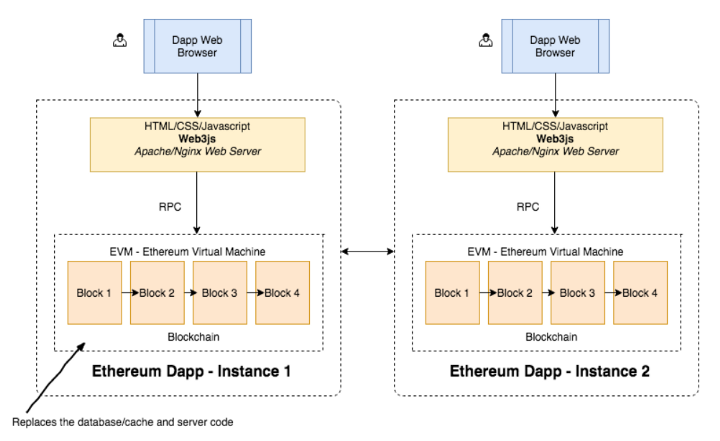
\includegraphics[width=1\textwidth]{ethereum_arquitectura.png}
     \caption{Arquitectura de Ethereum}. 
    \label{blockchain_ethereum_arquitecture}
\end{figure}

\noindent
\textbf{Hyperledger Fabric} \newline
Hyperledger Fabric presenta una arquitectura modular que permite implementaciones integrables de diversas funciones y herramientas. Uno de los elementos fundamentales del Fabric, es su ''protocolo de libro distribuido'', el cual es responsable de la integridad de datos en el \textit{blockchain} y es ejecutado por nodos. Aquí se diferencian 2 tipos de nodos:
\begin{itemize}
    \item Nodo Verificador: es un nodo en la red responsable de ejecutar el consenso, validar las transacciones y mantener el libro contable.
    \item Nodo No-Verificador: es un nodo que funciona como un proxy para conectar clientes (emitir transacciones) con nodos verificadores.
\end{itemize}

Como se mencionó en la sección de mecanismos de consenso, los ''nodos verificadores'' realizan un protocolo a prueba de ''fallas bizantinas'' para ejecutar una máquina de estado distribuido la cual acepta tres tipos de transacciones: implementación, invocación y consulta. La primera, hace referencia a la instalación de un chaincode dentro de un nodo; la segunda ejecuta el chaincode previamente instalado en el nodo (generando posibles cambios de estado) y la última, se refiere a la consulta de estado actual sobre el \textit{blockchain}.

Al estar enfocado en la implementación de libros contables autorizados, Fabric admite la autorización de inscripción y uso de transacciones a través de certificados de clave pública, y la confidencialidad para el chaincode (contratos inteligentes) ejecutados a través de cifrado \textit{in-band}.

En la Figura~\ref{blockchain_fabric_arquitecture}, se visualiza un ejemplo de aplicación de cuidados médicos soportada en Fabric. De lado derecho se aprecia su configuración física, del lado derecho sus componentes lógicos: permisología, nodos, consenso.

\begin{figure}[H]
    \centering
    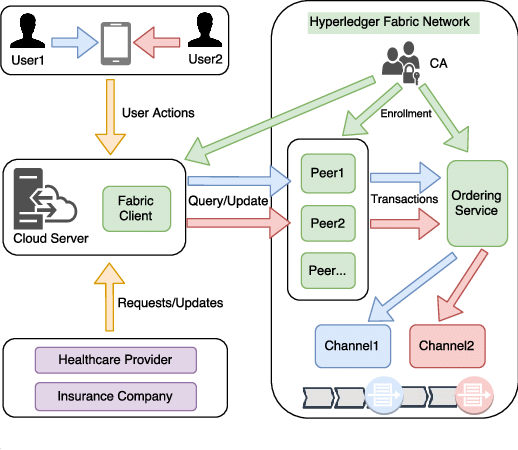
\includegraphics[width=0.8\textwidth]{fabric-arquitectura.png}
     \caption{Arquitectura de Fabric.} 
    \label{blockchain_fabric_arquitecture}
\end{figure}

Finalmente se presenta una tabla comparativa en la Figura ~\ref{blockchain_ethereum_hyperledger}  entre las dos plataformas con las características mas relevantes.

\begin{figure}[H]
    \centering
    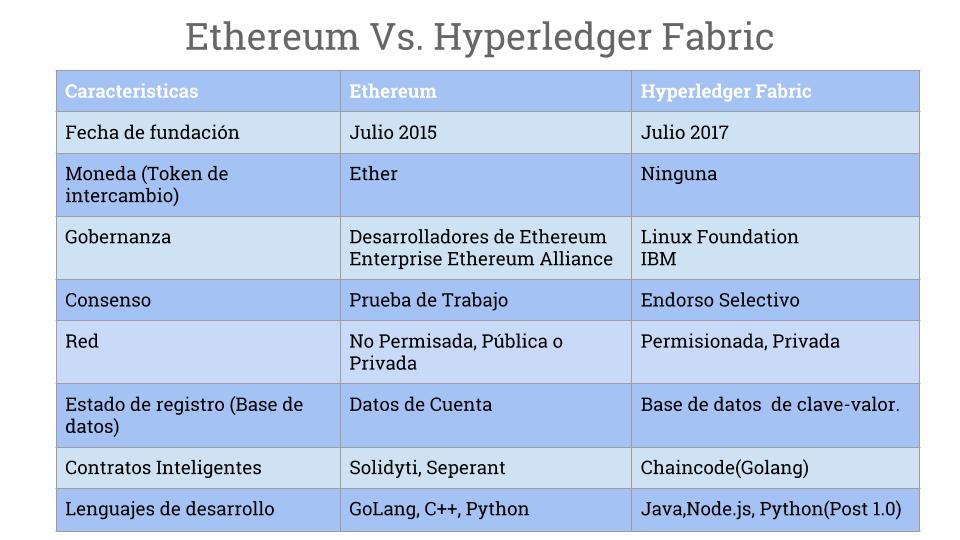
\includegraphics[width=1\textwidth]{Figs/Chapter2/ethereum_vs_hyperledger.jpg}
     \caption{Ethereum Vs. Hyperledger Fabric.} 
    \label{blockchain_ethereum_hyperledger}
\end{figure}

